%!TEX root=./Emile.tex
\section[Prolog: Rousseau]{Prolog: Rousseaus idealistisches Gedankenexperiment}

\epigraph{
	``Man was born free and yet everywhere he lives in chain stores.''\\*
	\emph{Jean-Jacques Rousseau / l`Internet}
}

Wie kann man Sozialwissenschaften und Pädagogik zusammen denken?
Wie persönliche Autonomie und inhärente Gleichheit verbinden?
Viele der Fragen, mit denen sich unserer Kurs beschäftigt, stellte sich Rousseau bereits im 18. Jahrhundert.
Auch wenn uns die Antworten, die er im \emph{Contrat Sociale} \parencite{Rousseau-1762-b} und dem Erziehungsroman \emph{Émile} \parencite{Rousseau1762} gibt, nicht unbedingt befriedigen mögen, so helfen sie doch zu präzisieren, wovon unser Kurs handelt.

\begin{dsafigurewide}[top]
	\begin{center}
	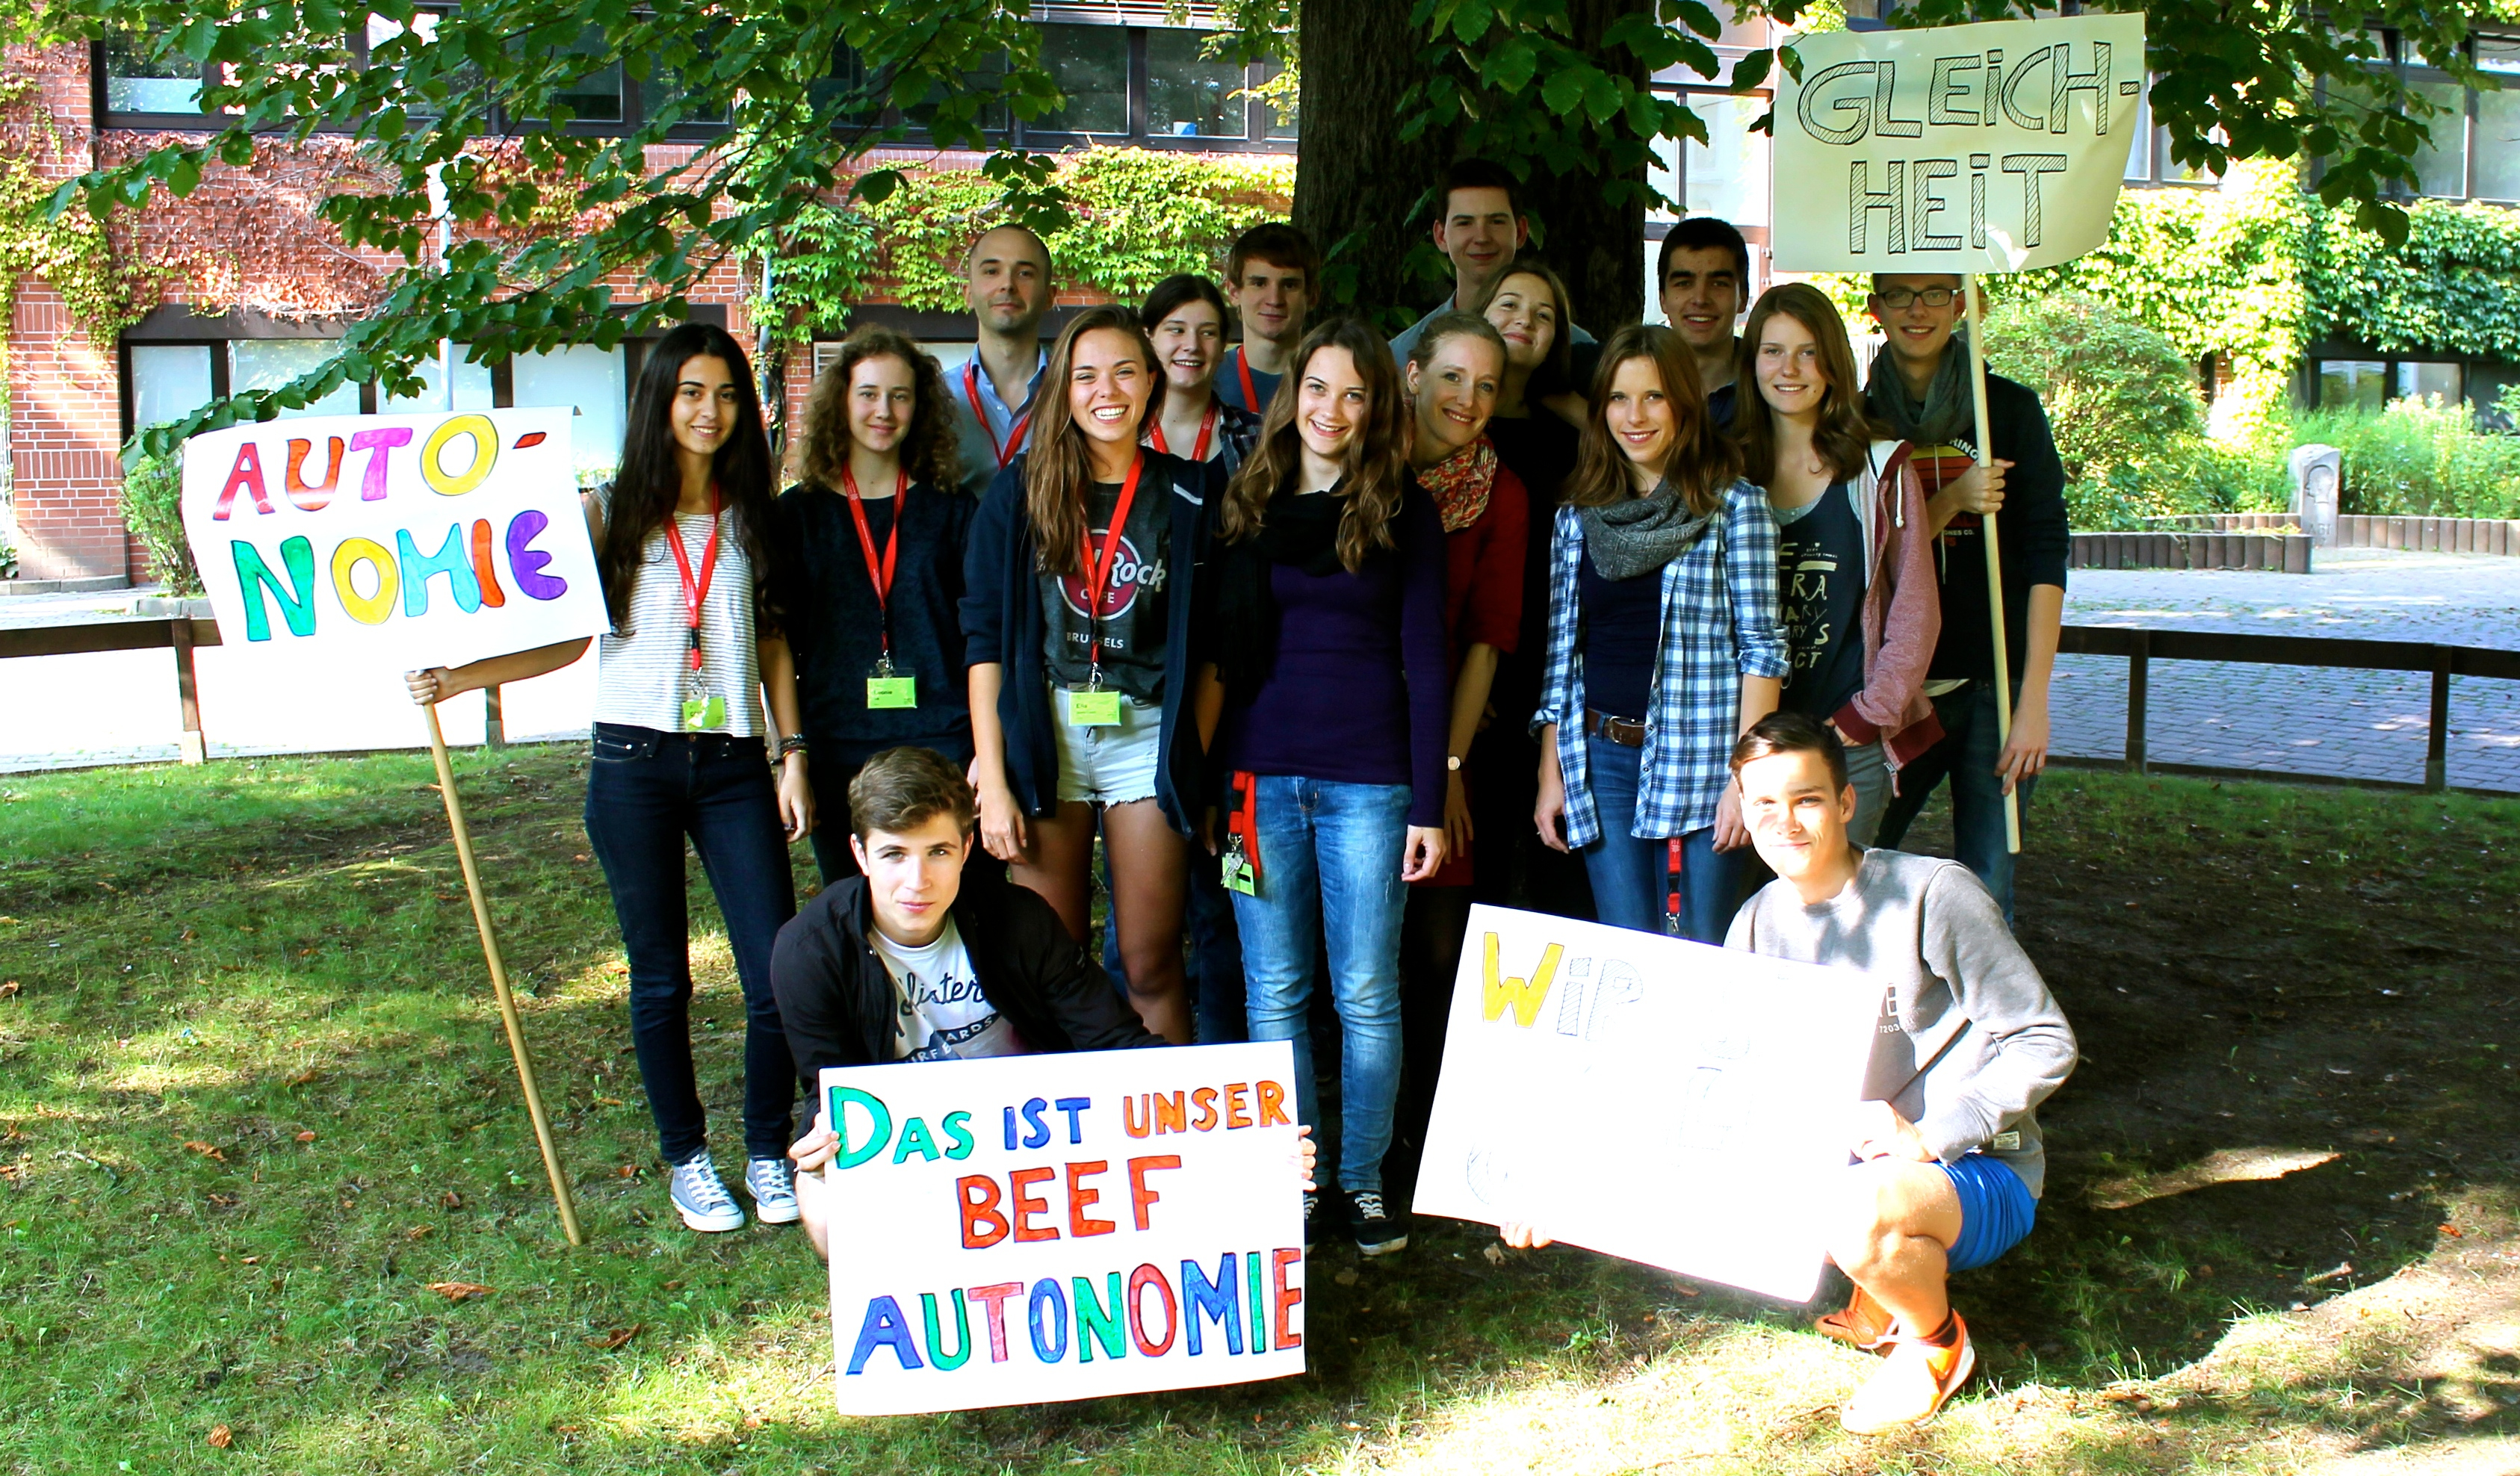
\includegraphics[width=.9\textwidth]{img/2014-2-4-Kursbild.jpg}
	\caption{Kurs 2.4}
	\label{fig:meinbild}
	\end{center}
\end{dsafigurewide}


\subsection{Émile: Oder über die Erziehung}

Rousseaus Gesellschaftsverständnis baut auf dem Menschenbild auf, das er in seinem Erziehungsroman Émile entwickelt:
Noch vor der französischen Revolution oder der Unabhängigkeitserklärung der Vereinigten Staaten stellt er, Bürger eines absolutistischen Feudalsystems, die These auf, jeder Mensch sei frei, persönlich autonom und inhärent gleich.
Er schreibt: ``Der Mensch wird frei geboren, und überall ist er in Banden.'' \parencite[1]{Rousseau-1762-b}.
Doch wenn der Mensch nicht natürlich erzogen wird, werden diese Grundeigenschaften überdeckt.
Als Beispiel, wie diese natürliche Erziehung aussehen soll, legt Rousseau die Erziehung seines fiktiven Zöglings \emph{Émile} dar.

In der Kindheit wird der Junge, abgeschottet von der Gesellschaft, negativ erzogen.
Das heißt, das Kind lernt nichts über Moral, Religion, Ethik, ..., sondern es wird vor ``Laster[n] und [...] Irrtümern bewahr[t]'' \parencite[54]{rousseau-1762}.
Anstelle dessen tritt eine Art ``Laissez-faire''-Pädagogik:
Wenn das Kind etwa von ihm benötigte Gegenstände zerstört,
``[b]eeilt euch nicht, ihm andere zu geben; laßt es empfinden, wie unangenehm es ist, sie nicht zu haben.'' \parencite[54]{rousseau-1762}.

Bis zum zwölften Lebensjahr soll das Kind auf diese Weise leben, stark und gesund werden.
Ab dann beginnt man das Kind in Naturkunde zu unterrichten \parencite[55]{rousseau-1762}.
In diesem Unterricht aber hat die Lehrerin/Erzieherin nur die Aufgabe, Lernsituationen zu schaffen.
Sie soll nichts erklären, sondern den Zögling allein herausfinden und verstehen lassen \parencite[56]{rousseau-1762}.

Erst wenn das Kind erwachsen wird, beginnt man mit der positiven Erziehung:
Das Kind wird nicht mehr als Zögling, sondern als Freund behandelt und moralisch, gesellschaftlich und religiös unterwiesen.
Es ist nun in der Lage, eigene fundierte Entscheidungen --- wie etwa die Wahl seiner Religion --- zu treffen \parencite[60f.]{rousseau-1762}.

Bald darauf kommt die Zeit, dass Émile in die Gesellschaft eingeführt werden muss, da der Mensch nicht für immer allein bleiben kann \parencite[61]{rousseau-1762}.
Der jetzt Erwachsene hat die Fähigkeit erworben, auch in der Gesellschaft seine Aufgabe zu erfüllen und trotzdem Mensch zu bleiben:

\begin{quote}
	``In der natürlichen Ordnung sind die Menschen alle einander gleich.
	Ihr gemeinsamer Beruf ist: Mensch zu sein.''\\*
	\parencite[50]{rousseau-1762}.
\end{quote}

Was passiert aber mit derjenigen, die nicht natürlich erzogen wird?
\footnote{
	%MH TODO: hier scheint die erste weibliche Form zu sein; ggfs. unten stehende Gender-Formulierung anpassen.
	Im Folgenden verwenden wir die grammatikalisch weibliche Form.
	Gemeint sind immer Personen aller sozialen Geschlechter.
}
Ihre bürgerliche Erziehung zerteilt sie in verschiedene Rollen und Identitäten, deren verschiedenen Pflichten nicht miteinander zu vereinbaren sind.
Sie ist z.B.\ als Abgeordnete dem Fraktionszwang unterworfen, etwa für eine Steuer zu stimmen, und als Angehörige eines Berufsstandes muss sie dagegen sein.
Oder sie muss als Teilnehmerin der kursübergreifenden Musik (KüMu) zu einer Probe erscheinen und als Kursteilnehmerin Protokoll schreiben usw.
Dadurch, dass sie sich über verschiedene Aufgaben definiert, kann es leicht zu inneren Rollenkonflikten kommen.
%MH TODO: hier wäre nochmal ein Beispiel gut...


\subsection{Le Contrat Social}

Während die bürgerlich Erzogene also in jeder ihrer Rollen \emph{Partikularinteressen} hat, kann ein natürlicher Mensch, der nur Mensch ist, das allgemeine menschliche Interesse des \emph{volonté générale} erkennen.
Rousseau geht davon aus, dass es im volonté générale (dem Gemeinwillen) ein vom Individuum losgelöstes abstraktes Wohl der Menschheit gibt.
Nur dieses Wohl könne in einem staatlichen System absolute Freiheit und Gleichheit garantieren.
Die problematische Vereinbarkeit von Freiheit und Gleichheit ergibt sich widerrum für Rousseau erst in der Moderne, da \emph{institutionalisierte}, rollenmäßig ausdifferenzierte Kooperation den \emph{volonté générale} verdecken.
In der Moderne ist der Weg der Kooperation durch Traditionen, Gesetze oder anderes institutionaliserte Formen vorgeschrieben, und definiert sich weniger zwischen natürlichen, \emph{ganzheitlichen} Menschen, sondern z.B.\ zwischen als SchülerAkademie-Teilnehmerin (``TN'') und SchülerAkademie-Kursleiterin (``KL'').
Für Rousseau ist der Urzustand zwar das Optimum, jedoch ist dieser unwiederbringlich verloren.
Deshalb schlägt Rousseau den Weg über den volonté générale als Lösung vor.
Nur er kann und muss staatliche Gewalt rechtfertigen.

In einem so gelenkten Staat herrscht Gleichheit, da jedes Individuum und die Gesellschaft im Ganzen das Bestmögliche erhalten \parencite[7]{Rousseau-1762-b}.
Es herrscht gleichzeitig Freiheit, weil jedes Mitglied sich \emph{freiwillig} der Gemeinschaft vollständig unterordnet.
Im Zweifelsfall muss der Mensch jedoch auch dazu gezwungen werden, diese Freiheit wahrzunehmen.
Dabei gilt für ihn ``Each man [sic!] in giving himself to everyone gives himself to no-one.'' \parencite[7]{Rousseau-1762-b}.
Er bleibt also vollkommen autonom.

Rousseau hat damit innerhalb seines Gedankenkonstrukts eine Lösung des Vereinbarkeitsproblems von Autonomie und Gleichwertigkeit gefunden
Seine Intention lag dabei darin, ein normatives Gebilde zu errichten, nicht aber darin, eine Verfassung zu schreiben.
%MH TODO nochmal ausführen, welche verfassungsmäßigen Details hier etwa fehlen, und welche Konflikte (etwa Abstimmungsmodus) hier völlig unbearbeitet bleiben.
Dennoch hat er als \emph{erster Aufklärer}, der eine göttliche Ordnung bestritt, großen Anteil an den freiheitlich demokratischen Entwicklungen der Folgezeit.

Rousseaus romantisch verklärten Ansichten bereiten zwar einige Verständnisprobleme und Widersprüche, doch wir müssen festhalten, dass seine anti-modernen Ideen faszinieren und viele Anregungen für die weitere Arbeit mitgeben.
